% !TEX TS-program = xelatex
%
\documentclass[aspectratio=1610]{beamer}

\usetheme{metropolis}

\usepackage{fontspec}
\defaultfontfeatures{Ligatures=TeX}

\usefonttheme{professionalfonts}
\usepackage[familydefault,light]{Chivo}

\usepackage{graphicx}
\graphicspath{{assets/}}
\usepackage[export]{adjustbox}

\usepackage{color}
\definecolor{red}{RGB}{200,50,0}
\definecolor{green}{RGB}{0,150,60}

\usepackage{enumitem}
\setitemize{
  label=\usebeamerfont*{itemize item}
  \usebeamercolor[fg]{itemize item}
  \usebeamertemplate{itemize item}
}

\usepackage{amssymb}
\usepackage{listings}

\lstdefinelanguage{mCRL2}{
  basicstyle=\ttfamily,
  sensitive = true,
  keywords={act, proc, init},
  otherkeywords={+, .},
  keywordstyle=\color{green},
  comment=[l]{\%},
  commentstyle=\color[rgb]{0.6,0.6,0.6}\itshape,
}

\usepackage{tkz-graph}
\tikzset{vertex/.style = {shape=circle,draw,minimum size=1}}
\tikzset{edge/.style = {->,> = latex'}}

\hypersetup
{
  pdftitle   = {Process Calculi for Concurrency},
  pdfauthor  = {Michael Kaltschmid \& Markus Reiter}
}

\title{Process Calculi}
\subtitle{for Concurrency}
\author{Michael Kaltschmid \& Markus Reiter}
\date{}

\begin{document}
  \maketitle

  \begin{frame}{Outline}
    \begin{itemize}
      \item What is a Process Calculus?
      \item µ-Calculus
      \item ACP
      \item mCRL2
    \end{itemize}
  \end{frame}

  \begin{frame}{What is a Process Calculus?}
    \begin{itemize}
      \item approach for formally modelling concurrent systems
      \item tool for high-level description of interactions, communications and synchronizations between processes
      \item provides algebraic laws to allow analyzing and transforming process descriptions
      \item permits formal reasoning about equivalences between processes (e.g., using bisimulation)
    \end{itemize}
  \end{frame}

  \begin{frame}{Process Calculi}
    \begin{itemize}
      \item \textbf{ACP}
      \item CCS
      \item CSP
      \item Join-Calculus
      \item \textbf{µ-Calculus}
      \item PEPA
      \item π-Calculus
    \end{itemize}
  \end{frame}

  \begin{frame}{Labelled Transition Systems}
    \begin{itemize}
      \item directed labelled graph \\
      \item consists of a set of state and a set of transitions labelled with actions that connect the states \\
      \item must have an initial state \\
      \item deadlock if a reachable state does not terminate and has no outgoing transitions \\
    \end{itemize}
  \end{frame}

  \begin{frame}{Labelled Transition Systems}
    LTS is a tuple $(S, A, \to,s_0>)$ where: \\[12pt]
    \begin{itemize}
      \item $S$ is a set of states \\
      \item $A$ is a set of actions \\
      \item $\to\ \subseteq S \times A \times S$ is a transition relation \\
      \item $s_0 \in S$ is the initial state \\
    \end{itemize}
    \begin{tabular}{cc}
      \begin{minipage}{.5\linewidth}
        \centering
        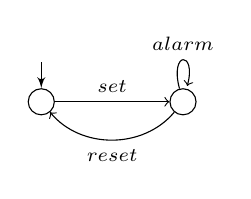
\begin{tikzpicture}[font=\sffamily\scriptsize]
          \node[vertex] (a) at (0, 0) {};
          \node[vertex] (b) at (1.8, 0) {};

          \draw[edge] (0, 0.5) to (a);
          \path[->] (a) edge  node[above] {$set$} (b);
          \path[->] (b) edge  [loop above] node {$alarm$} ();
          \path[->] (b) edge  [bend left=50] node[below] {$reset$} (a);
        \end{tikzpicture}
      \end{minipage}
      \begin{minipage}{.5\linewidth}
        \centering
        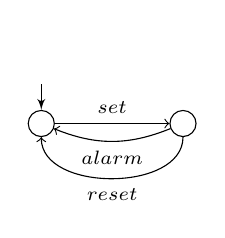
\begin{tikzpicture}[font=\sffamily\scriptsize]
          \node[vertex] (a) at (0, 0) {};
          \node[vertex] (b) at (1.8, 0) {};
          \node at (0, 1.1) {};

          \draw[edge] (0, 0.5) to (a);
          \path[->] (a) edge  node[above] {$set$} (b);
          \path[->] (b) edge  [bend left=22] node[below] {$alarm$} (a);
          \path[->] (b) edge  [bend left=90] node[below] {$reset$} (a);
        \end{tikzpicture}
      \end{minipage}
    \end{tabular}
  \end{frame}

  \begin{frame}{Bisimulation}
    Binary relation between LTSs, where LTSs behave the same way in the sense that one LTS simulates the other and vice versa. \\[24pt]

    \begin{exampleblock}{Trace equivalence:}
      Two LTSs are equivalent iff they can perform the same sequences of actions, starting from their initial states.
    \end{exampleblock}

    \begin{exampleblock}{Strong bisimilarity:}
      If one LTS can perform an action $a$ then the other LTS must also be able to perform an action $a$ in a way that the resulting states are again related.
    \end{exampleblock}
  \end{frame}

  \begin{frame}{Bisimulation}
    Bisimilarity of two coffee machines: \\[24pt]
    \centering
    \resizebox{\textwidth}{!}{
      \begin{tabular}{cc}
          \begin{tikzpicture}[font=\sffamily\tiny]
            \node[vertex] (P1) at (1.6, 3) {$P1$};
            \node[vertex] (P2) at (1.6, 1.7) {$P2$};
            \node[vertex] (P3) at (3.2, 0) {$P3$};
            \node[vertex] (P4) at (0, 0) {$P4$};

            \path[edge] (P1) edge node[fill=bg] {$insert\ coin$} (P2);
            \path[edge] (P2) edge node[fill=bg] {$choose\ coffee$} (P3);
            \path[edge] (P2) edge node[fill=bg] {$choose\ tea$} (P4);
            \path[edge] (P3) edge [bend right=40] node[fill=bg] {$pour\ coffee$} (P1);
            \path[edge] (P4) edge [bend left=40] node[fill=bg] {$pour\ tea$} (P1);
          \end{tikzpicture}
          &
          \begin{tikzpicture}[font=\sffamily\tiny]
            \node[vertex] (Q1) at (1.6, 3) {$Q1$};
            \node[vertex] (Q2) at (0, 1.7) {$Q2$};
            \node[vertex] (Q3) at (3.2, 1.7) {$Q3$};
            \node[vertex] (Q4) at (0, 0) {$Q4$};
            \node[vertex] (Q5) at (3.2, 0) {$Q5$};

            \path[edge] (Q1) edge node[fill=bg] {$insert\ coin$} (Q2);
            \path[edge] (Q1) edge node[fill=bg] {$insert\ coin$} (Q3);
            \path[edge] (Q2) edge node[label=left:$choose\ tea$] {} (Q4);
            \path[edge] (Q3) edge node[label=right:$choose\ coffee$] {} (Q5);
            \path[edge] (Q4) edge [bend right=25] node[fill=bg] {$pour\ tea$} (Q1);
            \path[edge] (Q5) edge [bend left=25]  node[xshift=7.5pt, yshift=-10pt, fill=bg] {$pour\ coffee$} (Q1);
          \end{tikzpicture}
      \end{tabular}
    }
  \end{frame}

  \begin{frame}{µ-Calculus – Hennessy-Milner Logic}
    \begin{align*}
      af ::= \alpha\ |\ true\ |\ false\ |\ \neg \phi\ |\ \phi \land \psi\ |\ \phi \lor \psi\ |\ \phi \to \psi\ |\ \langle a \rangle \phi \ |\ [a]\phi
    \end{align*}
    \begin{itemize}
      \item $\neg ,\ \land\ ,\ \lor$ and $\to$ as usual
      \item $\langle a \rangle \phi$ is valid whenever an $a-action$ can be performed such that $\phi$ is valid after this $a$ has been done
      \item $[a]\phi$ is valid when for every action $a$ that can be done, $\phi$ holds after doing that $a$
    \end{itemize}
  \end{frame}

  \begin{frame}{µ-Calculus – Diamond \& Box Modalities}
    \resizebox{\textwidth}{!}{
      \newcommand{\valid}{{\color{green} valid}}
      \newcommand{\invalid}{{\color{red} invalid}}
      \renewcommand{\arraystretch}{2}
      \begin{tabular}{l c c c c}
        &

        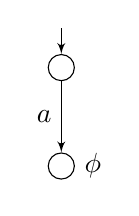
\begin{tikzpicture}
          \node[vertex] (a) at (0, 1.25) {};
          \node[vertex] [label=right:{$\phi$}] (b) at (0, 0) {};

          \draw[edge] (0, 1.75) to (a);
          \draw[edge] (a) to node [left] {$a$} (b);
        \end{tikzpicture}

        &

        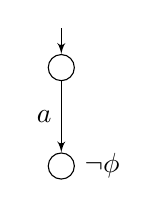
\begin{tikzpicture}
          \node[vertex] (a) at (0, 1.25) {};
          \node[vertex] [label=right:{$\neg\phi$}] (b) at (0, 0) {};

          \draw[edge] (0, 1.75) to (a);
          \draw[edge] (a) to node [left] {$a$} (b);
        \end{tikzpicture}

        &

        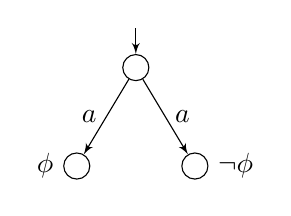
\begin{tikzpicture}
          \node[vertex] (a) at (0.75, 1.25) {};
          \node[vertex] [label=left:{$\phi$}] (b) at (0, 0) {};
          \node[vertex] [label=right:{$\neg\phi$}] (c) at (1.5, 0) {};

          \draw[edge] (.75, 1.75) to (a);
          \draw[edge] (a) to node [left] {$a$} (b);
          \draw[edge] (a) to node [right] {$a$} (c);
        \end{tikzpicture}

        &

        \begin{tikzpicture}
          \node[vertex] (a) at (0, 1.25) {};
          \node at (0, -0.175) {};

          \draw[edge] (0, 1.75) to (a);
        \end{tikzpicture}

        \\

        $\langle{}a\rangle{}\phi$ & \valid & \invalid & \only<-1>{\phantom{\valid}}  \only<2->{\valid}   & \only<-3>{\phantom{\invalid}} \only<4->{\invalid} \\

        $[a]\phi$                 & \valid & \invalid & \only<-2>{\phantom{\invalid}}\only<3->{\invalid} & \only<-4>{\phantom{\valid}}   \only<5->{\valid}   \\
      \end{tabular}
    }
  \end{frame}

  \begin{frame}{µ-Calculus – Regular Formulae}
    \begin{itemize}
      \item allow more than a single action in a modality
      \item useful for expressing that after two or more \\
            arbitrary actions, a specific action must happen
      \item based on action formulae
    \end{itemize}

    \begin{exampleblock}{A more concrete example:}
      After two \textit{\textbf{receive}} actions, a \textit{\textbf{send}} action must follow.
    \end{exampleblock}
  \end{frame}

  \begin{frame}{µ-Calculus – Action Formulae}
    An action formula $af$ defines a set of multi-actions.

    \begin{align*}
      af ::= \alpha\ |\ true\ |\ false\ |\ \overline{af}\ |\ af\ \cap\ af\ |\ af\ \cup\ af
    \end{align*}

    \begin{itemize}
      \item $\alpha$ represents the set with exactly the multi-action $\alpha$.
      \item $true$ is the set of all multi-actions.
      \item $false$ is the empty set.
      \item $\overline{af}$ denotes the complement of the set $af$.
      \item $\cup$ and $\cap$ denote union and intersection, respectively.
    \end{itemize}
  \end{frame}

  \begin{frame}{µ-Calculus – Action Formulae}
    $af$ being a set of multi-actions, modalities with action formulae are defined like this:

    \begin{align*}
      \langle{af}\rangle\phi = \bigvee_{\alpha \in af} \langle\alpha\rangle\phi
      \qquad\qquad
      [af]\phi = \bigwedge_{\alpha \in af} [\alpha]\phi
    \end{align*}

    \begin{exampleblock}{Example}
      \begin{itemize}
        \item $\langle\overline{a}\rangle\langle{b \cup c}\rangle{true}$ means an action other than $a$ can be done, followed by either $b$ or $c$.
        \item $[\overline{a}]false$ says that only an $a$ action is allowed.
      \end{itemize}
    \end{exampleblock}
  \end{frame}

  \begin{frame}{µ-Calculus – Regular Formulae}
    Regular formulae extend action formulae, allowing sequences of actions in modalities.

    \begin{align*}
      R ::= \epsilon\ |\ af\ |\ R\cdot{R}\ |\ R+R\ |\ R^*\ |\ R^+
    \end{align*}

    \begin{itemize}
      \item $\epsilon$ is the empty sequence of actions.
      \item $R_1\cdot{R_2}$ represents the concatenation of $R_1$ and $R_2$.
      \item $R_1+R_2$ denotes the union of  $R_1$ and $R_2$.
      \item $R^*$ denotes zero ore more repetitions.
      \item $R^+$ denotes one ore more repetitions.
    \end{itemize}
  \end{frame}

  \begin{frame}{µ-Calculus – Regular Formulae}
    \begin{exampleblock}{Examples}
      \begin{itemize}
        \item $[\epsilon]\phi = \langle\epsilon\rangle\phi = \phi$, so one can always perform no action, and remain in the same state.
        \item $\langle{a}\cdot{b}\cdot{c}\rangle{true}$ is the same as $\langle{a}\rangle\langle{b}\rangle\langle{c}\rangle{true}$.
        \item $[a\cdot{b} + c\cdot{d}]false$ means that neither the sequence $a\cdot{b}$ nor $c\cdot{d}$ is possible.
        \item $\langle{a^*}\rangle{true}$ expresses that any sequence of $a$ actions is possible.
        \item $[a^+]\phi$ says that $\phi$ must hold in any state reachable by one or more $a$ actions.
      \end{itemize}
    \end{exampleblock}
  \end{frame}

  \begin{frame}{µ-Calculus – Regular Formulae}
    Two other commonly used formulae are the \textit{always} and \textit{eventually} modalities.

    \begin{align*}
      \square\phi = [true^*]\phi \qquad\qquad    \diamond\phi = \langle{true^*}\rangle\phi
    \end{align*}

    \begin{itemize}
      \item $\square\phi$ means that $\phi$ holds in all reachable states.
      \item $\diamond\phi$ says that there is a sequence of actions after which $\phi$ holds.
    \end{itemize}
  \end{frame}

  \begin{frame}{µ-Calculus – Regular Formulae: Safety Property}
    \begin{align*}
      \square\phi \implies \text{Something bad will never happen.}
    \end{align*}

    \begin{exampleblock}{Example}
      We have a program with a critical region and two actions, \textit{enter} and \textit{leave}.

      \begin{align*}
        [true^*\cdot enter \cdot \overline{leave}^* \cdot enter]false
      \end{align*}

      It is impossible to enter twice in a row. There has to be a \textit{leave} action in between two \textit{enter} actions.
    \end{exampleblock}
  \end{frame}

  \begin{frame}{µ-Calculus – Regular Formulae: Liveness Property}
    \begin{align*}
      \diamond\phi \implies \text{Something good will happen.}
    \end{align*}

    \begin{exampleblock}{Example}
      \begin{align*}
        [true^*\cdot send]\langle true^* \cdot receive \rangle true
      \end{align*}

      Every time a message is sent, it can eventually be received.
    \end{exampleblock}
  \end{frame}

  \begin{frame}{µ-Calculus – Fixed Point Modalities}
    By extending the Hennessy-Milner logic with fixed points we have:
    \resizebox{ \textwidth}{!} {
      \begin{minipage}{\textwidth}
        \begin{align*}
          af ::= \alpha\ |\ true\ |\ false\ |\ \neg \phi\ |\ \phi \land \psi\ |\ \phi \lor \psi\ |\ \phi \to \psi\ |\ \langle a \rangle \phi \ |\ [a]\phi\ |\ \color{green} \mu X. \phi \ |\ vX. \phi \ |\ X.
        \end{align*}
      \end{minipage}
    }
    \begin{itemize}
      \item $X$ is a set of states
      \item $\mu X. \phi$ is the minimal fixed point
      \item $vX. \phi$ is the maximal fixed point
      \item minimal and maximal fixed point operators are each other's duals
    \end{itemize}
    \begin{tabular}{cc}
      \begin{minipage}{.47\linewidth}
        \begin{align*}
          \neg vX. \phi = \mu X. \neg \phi
        \end{align*}
      \end{minipage}
      \begin{minipage}{.47\linewidth}
        \begin{align*}
          \neg \mu X. \phi = vX. \neg \phi
        \end{align*}
      \end{minipage}
    \end{tabular}
  \end{frame}

  \begin{frame}{µ-Calculus – Fixed Point Modalities}
    \begin{exampleblock}{Example}
      \begin{center}
        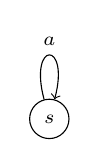
\begin{tikzpicture}[font=\sffamily\scriptsize]
          \node[vertex] (S) at (0, 0) {$s$};
          \path[->, every loop/.style={looseness=15}] (S) edge  [loop above] node {$a$} ();
        \end{tikzpicture}
      \end{center}
      \begin{itemize}
        \item Do $\mu X. \langle a \rangle X$ and $vX. \langle a \rangle X$ hold for the state $s$?
        \item states to consider: empty set $X = \emptyset$ and set of all states $X = \{s\}$
        \item if $X = \emptyset$ then $X = \langle a \rangle X$ reduces to $false = \langle a \rangle false$, which is valid
        \item $\mu X. \langle a \rangle X$ is valid for all states in the empty set but not in $s$
        \item $vX. \langle a \rangle X$ is valid for all states in the largest set $\{s\}$
      \end{itemize}
    \end{exampleblock}
  \end{frame}


  \begin{frame}{Algebra of Communicating Processes (ACP)}
    \begin{align*}
      P ::= a\ |\ \delta\ |\ \tau\ |\ P + P\ |\ P \cdot P\ |\ (P || P)\ |\ (P |\lfloor P)\ |\ (P | P)\ |\ \tau_I(P)
    \end{align*}

    \begin{itemize}
      \item $a$ represents an atomic action, $\delta$ is the deadlock action \\ and $\tau$ is the silent action.
      \item $a + b$ means either $a$ or $b$ (a.k.a. \textit{alternative operator}).
      \item $a \cdot b$ means $a$ followed by $b$ (a.k.a. \textit{sequencing operator}).
      \item $||$ denotes concurrency (a.k.a. merge operator).
      \item $|\lfloor$ is a special case of $||$ (a.k.a. \textit{left-merge operator}).
      \item $|$ is the communications operator.
      \item $\tau_I$ is the abstraction operator, used to “hide” certain actions.
    \end{itemize}
  \end{frame}

  \begin{frame}{Algebra of Communicating Processes (ACP)}
    \begin{exampleblock}{Examples}
      \begin{itemize}
        \item $(a \cdot b) || (c \cdot d)$ means $a \cdot b$ in parallel with $c \cdot d$, so either $abcd$, $acbd$, $acdb$, $cabd$, $cadb$ or $cdab$.
        \item $(a \cdot b) |\lfloor (c \cdot b)$ ensures that the left branch is started first, in this case that $a$ occurs first, \\ so only $abcd$, $acdb$ and $adbc$ are possible.
        \item $r(d) | w(d)$ means that the value $d$ is communicated from action $w$ from the right side to $r$ on the left side (a.k.a. communications operator).
        \item $\tau_{\{c\}}((a+b)\cdot c) = (a + b) \cdot \tau$, which can be reduced to $a + b$.
      \end{itemize}
    \end{exampleblock}
  \end{frame}

  \begin{frame}{mCRL2}
    \begin{itemize}
      \item formal specification language for processes
      \item based on ACP
      \item uses µ-Calculus for model checking
      \item used for specifying and analysing behaviour of distributed systems and protocols
    \end{itemize}
  \end{frame}

  \begin{frame}[fragile]{mCRL2: Syntax}
    \begin{lstlisting}[language=mCRL2]
% Actions
act a, b, c, d, e;

% Processes
proc P = a . b . c;           % Sequence
     Q = d + e;               % Alternative
     R = (a + b) . c . d . e; % Alternative & Sequence

% Specify that the process starts with process P.
init P;
    \end{lstlisting}
  \end{frame}

  \begin{frame}[standout]
    mCRL2 Live Demo
  \end{frame}

  \begin{frame}[standout]
    Why do we need this?
  \end{frame}

  \begin{frame}{Real-World Example: Automated Parking Garage}
    \begin{tabular}{cc}
      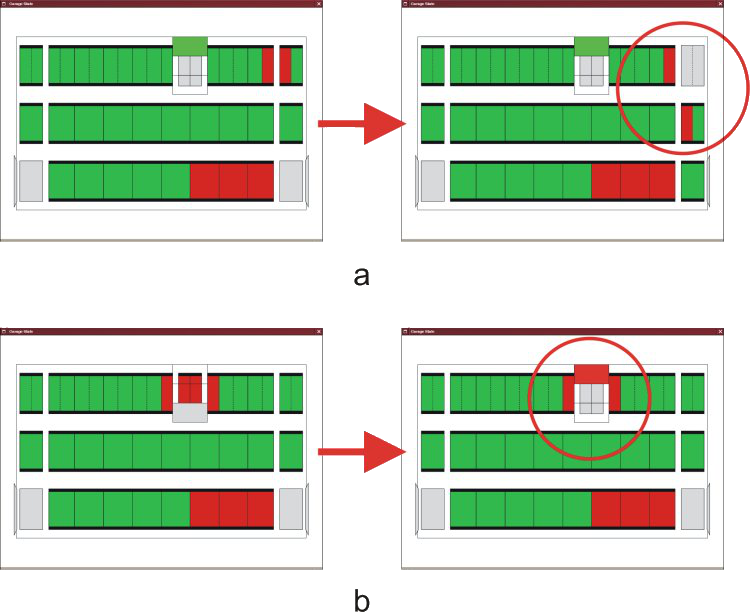
\includegraphics[width=0.475\textwidth, valign=t]{parking_garage_errors.png}
      &
      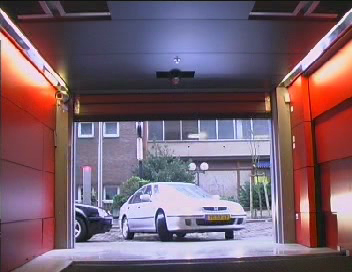
\includegraphics[width=0.465\textwidth, valign=t]{parking_garage_enter.png}
    \end{tabular}

    \begin{enumerate}[label=(\alph*)]
      \item It was possible to rip a car in half with the shuttles.
      \item It was possible to damage two cars using the lift.
    \end{enumerate}
  \end{frame}
\end{document}
